%%% DOCUMENT SETUP %%%
\documentclass[11pt,a4paper,onecolumn]{article}
\usepackage[english]{babel}

%%% LAYOUT %%%
\usepackage{fullpage}
\usepackage[a4paper]{geometry}
\usepackage[parfill]{parskip}
\usepackage{multicol}
\usepackage{footnote}

%%% GRAPHICS %%%
\usepackage{graphicx}
\usepackage{color}
\usepackage{graphics}
\usepackage{rotating}
\usepackage{subfig}
\usepackage{amsmath}
\usepackage{amssymb}
\usepackage{amscd}
\usepackage{xfrac}
\usepackage{float}
\usepackage{dsfont}

%%% FONT %%%
\usepackage{ifxetex}
\ifxetex
  \usepackage{fontspec}
    \setmainfont{Linux Libertine O}
  \usepackage{xunicode}
  \usepackage{microtype}
\else
  \usepackage[T1]{fontenc}
  \usepackage[latin1]{inputenc}
  \usepackage{times}
  \usepackage{microtype}
\fi

%%% Coding %%%
\usepackage{listings}
\usepackage{pseudocode}

%%% TITLE PAGE %%%
\author{Jeroen Hofman (10194754) \\
[15pt] University of Amsterdam (\textsc{UvA})}

\title{Concurrent Programming week 3:\\
  OpenMP
		}

\begin{document}
\maketitle
\captionsetup{width=0.8\textwidth}
\lstset{language=C,breaklines=true,backgroundcolor=\color{white},frame=none,basicstyle=\footnotesize}
\thispagestyle{empty}

%%% ABSTRACT %%%
\begin{center}
\begin{abstract}
\small{We performed a parallelisation of the heat diffusion code with OpenMP. We found linear speedups but poor performance when comparing the multithreaded code with 1 thread to the sequential code, most likely because of 'false sharing' or some other unidentified error. Furthermore we look at different scheduling options and found the dynamic scheduling option most efficient for the problem at hand. We also parallelised a piece of code with OpenMP.}
\end{abstract}
\end{center}

%%% TABLE OF CONTENTS %%%
\newpage
\tableofcontents
\newpage

\section{Introduction}

\section{Heat diffusion with OpenMP}
\subsection{Algorithm}
The algorithm is nearly the same in structure as for Pthreads, only some parts of the code set up are scrambled (see /omp/compute.c). After initialization and starting the timer a \texttt{parallel} is created (we omit \texttt{\# pragma omp} in the rest of this report). In this \texttt{parallel} the main loop is started, iterations in this loop are dependent upon previous iterations, so this loop cannot be parallelised. All threads have a local variable \emph{diff}, the temperature difference, set to zero at every iteration. The threads then proceed with doing the main computation with a \texttt{for}, filling the new temperature array and calculating the local maximum of \emph{diff} with a \texttt{static} workload distribution. The threads do not synchronize after this main computation because this is not needed. After the main computation the local value of \emph{diff} is written to a global variable \emph{maxdiff}. This is done by first checking if the local variable is larger than the global value, because we are interested in the maximum. If this is the case, the thread enters a critical region where it checks again if the condition holds, and writes \emph{diff} to the global variable \emph{maxdiff}. The double checking is done because it prevents threads from going into a critical region to often. The inner check cannot be left out since another thread can have written something to the global variable in the meantime and hence the checked condition might no longer be valid.

Next the threads enter a part of the code where the results are computed, this will occur if the iteration number is a multiple of the report frequency. If reporting is needed, each thread calculates a local maximum and minimum temperature with a \texttt{for} compiler annotation. They also calculate the average temperature \emph{avg}, since this is a simple operation this is done with a reduction in \texttt{for}, and hence \emph{avg} is global. Reduction for double data types does not work properly, as there are small rounding differences between different number of threads as input, this has also be observed by others \cite{chandra}. After having computed the local maximum and minimum temperature, the threads write these to the global variables, again by entering a \texttt{critical}. The construct with the double if statement around \texttt{critical} is not used in this case since reporting is not executed often and mostly used for debugging.

After completing the intermediate report step (or skipping it) the next action performed is copying the columns, this can only be done after all threads have finished their main computation to create the new temperature matrix, since otherwise some values might not have been computed yet and copying will then provide wrong values for the halo columns. For this purpose a barrier is implemented. However, there is no difference in results between omitting this barrier or not, indicating that most likely each thread is assigned the same rows both for the main iteration and for the copying of the columns, in which case the above does not apply. This is however implementation dependent, so the barrier is still implemented in the code.

After the threads have finished copying columns a single thread reports the earlier computed results by using \texttt{single}. This thread also performs swapping of arrays and initializes the variables for the next iteration. This could also be done separately by using \texttt{section} but since the operations only involve swapping pointers and setting variables, the overhead created by using \texttt{section} is much larger than the benefit of having these operations performed concurrently.

As before, after the computation has reached the maximum amount of iterations or reaches the threshold, the for loop is terminated and the threads do one final (parallelised) computing of results and reporting, similar as described for the intermediate reporting.

This code has three implicit barriers, instead of two in the Pthread-code. One barrier after the main computation, another after the copying of the halo columns and the last one after reporting, swapping and initializing variables. The extra barrier with respect to Pthreads is the first one, since with Pthreads one can manually implement that threads handle the same part of the matrix throughout the code. However with OpenMP one does not have control over this.

\subsection{Results}
Like the last report, we report execution times and FLOP/s (using the original macro) for different matrix sizes and numbers of threads. The best performance over 3 runs was taken. Relative speedups are given in Figure \ref{fig:heat} where the solid line has the sequential line as basecode and the dashed line has the multithreaded code with 1 thread as baseline. Table \ref{tab:heat} gives the exact results. All computations are performed on a LISA node with 8 cores.

\begin{figure}[H]
  \centering
  \subfloat{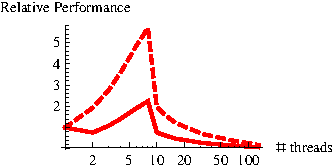
\includegraphics[width=0.33\textwidth]{100.pdf}}
  \subfloat{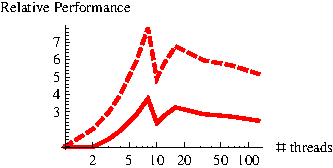
\includegraphics[width=0.33\textwidth]{1000.pdf}}
  \subfloat{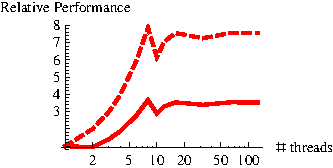
\includegraphics[width=0.33\textwidth]{5000.pdf}}
  \caption{Relative performance results for matrix size 100x100 (left), 1000x1000 (middle) and 5000x5000 (right). The solid line has the sequential code as baseline, the dashed line has the multithreaded code with 1 thread as baseline.}
  \label{fig:heat}
\end{figure}

\begin{table}[H]
  \centering
  \begin{tabular}{l | c | l | c | l }
    \# threads & Execution time & FLOP/s & Execution time & FLOP/s \\
    \hline
    \multicolumn{1}{c}{} & \multicolumn{2}{| c |}{Size 100x100 ($10^6$ iterations)} & \multicolumn{2}{c}{Size 1000x1000}\\
    \hline
    seq. code & 53.130341 & 2.258596 $10^9$ & 6.353987 & 1.888578 $10^9$ \\
    1 & 11.199501 & 8.888646  $10^8$ & 13.293972 & 9.026648 $10^8$ \\
    2 & 5.791749 & 1.718797 $10^9$ & 6.626487 & 1.810914 $10^9$ \\
    3 & 4.023621 & 2.474100 $10^9$ & 4.434140 & 2.706275 $10^9$ \\    
    4 & 3.137461 & 3.172897 $10^9$ & 3.326681 & 3.607199 $10^9$ \\
    6 & 2.303877 & 4.320908 $10^9$ & 2.234351 & 5.370687 $10^9$ \\
    8 & 1.965309 & 5.065280 $10^9$ & 1.693954 & 7.084017 $10^9$ \\
    10 & 5.732374 & 1.736600  $10^9$ &2.704565 & 4.436943  $10^9$ \\
    12 & 6.854336 & 1.452342 $10^9$ & 2.296002 & 5.226476 $10^9$ \\
    16 & 9.219849 & 1.079718 $10^9$ & 1.956240 & 6.134216 $10^9$ \\
    32 & 16.390338 & 6.073603 $10^8$ &2.222420 & 5.399520  $10^9$ \\
    64 & 27.530701 & 3.615905 $10^8$ & 2.334190 & 5.140969 $10^9$ \\
    128 & 60.513910 & 1.645050 $10^8$ & 2.557037 & 4.692932 $10^9$ \\
    \hline
    \multicolumn{1}{c}{} & \multicolumn{2}{| c |}{Size 20000x500} & \multicolumn{2}{c}{Size 500x20000}\\
    \hline
    seq. code & 63.647849 & 1.885374 $10^9$ & 65.108231 & 1.843085 $10^9$ \\
    1 & 131.608427 & 9.117957 $10^8$ &133.165973 & 9.011311  $10^8$ \\
    2 & 66.025820 & 1.817471 $10^9$ & 66.592396 & 1.802008 $10^9$ \\
    3 & 44.041182 & 2.724723 $10^9$ &44.540139 & 2.694199  $10^9$ \\
    4 & 33.122345 & 3.622932 $10^9$ & 33.473068 & 3.584972 $10^9$ \\
    6 & 22.247607 & 5.393839 $10^9$ & 22.692589 & 5.288070 $10^9$ \\
    8 & 17.130007 & 7.005251 $10^9$ & 17.550506 & 6.837410 $10^9$ \\
    10 & 26.137627 & 4.591082 $10^9$ & 26.424073 & 4.541314 $10^9$ \\
    12 & 22.382556 & 5.361318 $10^9$ & 22.822582 & 5.257950 $10^9$ \\
    16 & 17.819982 & 6.734014 $10^9$ & 18.597260 & 6.452563  $10^9$ \\
    32 & 17.598885 & 6.818614 $10^9$ & 18.355196 & 6.537658 $10^9$ \\
    64 & 17.795912 & 6.743122 $10^9$ & 18.583452 & 6.457358 $10^9$ \\
    128 & 18.105109 & 6.627963 $10^9$ & 19.324433 & 6.209755  $10^9$ \\
    \hline
    \multicolumn{1}{c}{} & \multicolumn{2}{| c |}{Size 5000x5000} & \multicolumn{2}{c}{}\\
    \hline
    seq. code & 155.836412 & 1.925096 $10^9$ & & \\
    1 & 332.849808 & 9.013074 $10^8$ & & \\
    2 & 166.300583 & 1.803962 $10^9$ & & \\
    3 & 110.995404 & 2.702815 $10^9$ & & \\
    4 & 83.332347 & 3.600043 $10^9$ & & \\
    6 & 55.818338 & 5.374578 $10^9$ & & \\
    8 & 42.368601 & 7.080715 $10^9$ & & \\
    10 & 54.021732 & 5.553321 $10^9$ & & \\
    12 & 47.246477 & 6.349680 $10^9$ & & \\
    16 & 44.029770 & 6.813572 $10^9$ & & \\
    32 & 45.862236 & 6.541330 $10^9$ & & \\
    64 & 43.977064 & 6.821738 $10^9$ & & \\
    128 & 44.144347 & 6.795887 $10^9$ & & \\
  \end{tabular}
  \caption{Results for the multithreaded code for heat diffusion for different matrix sizes and number of threads.}
  \label{tab:heat}
\end{table}

The results are similar to the results reported in the last report. The behavior as a function of size is exactly the same, so we will not repeat all these arguments (e.g. difference between 20000x500 and 500x20000 matrix, local maxima, minima). Again, the highest speedup is achieved for 8 threads, and high speedup is also seen for multiples of 8 threads. The speedup is almost linear for large matrix sizes and less for the 100x100 matrix, though it is still significant (unlike the case of Pthreads).

There is however one important remark, the multithreaded code with 1 thread is much slower than the sequential code, around 50\%, this is a feature that was absent with the Pthread implementation. This is also why Figure \ref{fig:heat} shows only a factor 4 increase when compared to the sequential code for 1000x1000 and 5000x5000. After testing the code it turned out that the bottleneck is the writing of the local maximum temperature difference \emph{diff} to a global variable \emph{maxdiff}, when this piece of code was omitted the code sped up with a factor 2 almost (and thereby being nearly as fast as the sequential code). This is the piece of code described above with the double embedded if-statement and the critical section. Even omitting this statements and the critical section and simply writing the local variable to the global (in the code this boils down literally to: maxdiff = diff;) is enough to slow down the code by 50\%, regardless of positioning of this simple line in the code. No solution has been found for this problem so far, as in some point in the code the threads have to communicate their values to a global variable. It might be a problem related to 'false sharing' as discussed in the lectures, but even with using the \texttt{flush} directive of OpenMP no significant performance increase was found.

Furthermore we find a peak performance of $7.08 \; 10^9$ for 1000x1000, which is slightly lower compared to the peak performance found for the code with Pthreads, which was $7.22 \; 10^9$ for a matrix of size 20000x500 and 8 threads. However, the OpenMP version contains some general optimizations not present in the Pthread version, so in that sense it is not a fair comparison. Also fixing the bug would give a major speedup compared to Pthreads.

\section{Scheduling types}
For this part of the assignment we look at different scheduling types used for a parallelisation of an upper triangular matrix where in a loop every element of the matrix is incremented by one. We parallelise the rows of the matrix. We use the following scheduling types for parallelising this problem:
\begin{itemize}
\item 
  Static: each thread is assigned a chunk of certain size in a round robin fashion beforehand. When no chunk size is specified the chunk size is roughly equal to the number of rows divided by the number of threads.
\item
  Dynamic: the same system as static, only which thread does which chunk is not determined beforehand, but chunks are given out whenever a thread has finished doing its previously assigned chunk.
\item
  Guided: Chunks are assigned of decreasing size in a dynamic way. The $k$-th chunk size is proportional to $e^{-ck}$ with $c$ some parameter \cite{chunk}. The first chunk is approximately equal to the loop size divided by the number of threads.
\end{itemize}

We tested this scheduling types for an upper triangular matrix of size 100x100, 1000x1000 and 5000x5000 for static scheduling, dynamic default (1), 5, 10 and 20 and guided 1, 2, 3 (1000 iterations). The results are shown in Figure \ref{fig:chunks} below. The measurements are made on a LISA node with 8 cores.

\begin{figure}[H]
  \centering
  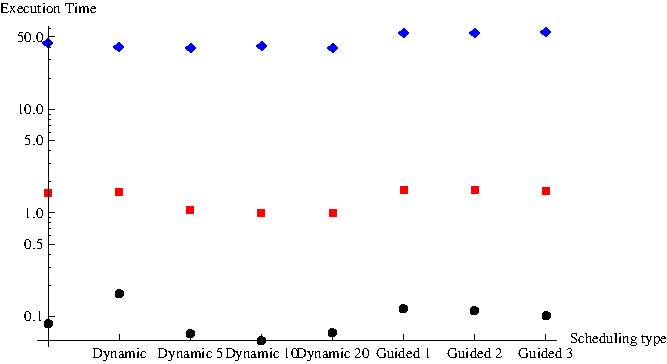
\includegraphics[width=0.7\textwidth]{chunks.pdf}
  \caption{Execution time for different scheduling types (outer left is static), black is for size 100x100, red for 1000x1000 and blue for 5000x5000.}
  \label{fig:chunks}
\end{figure}

For all three problem sizes the best performance is achieved with the dynamic 20 scheduling. The guided scheduling performs the worst overall. This is strange since the workload of this problem is not balanced and hence the guided scheduling would at first thought be the preferred scheduling. The static scheduling also performs badly for this same reason. The speedup for dynamic scheduling is achieved because the threads are used in a very efficient way, whenever one is finished it gets assigned a new piece right away, such that no thread is suspended, unlike the static case. 

A possible explanation of the poor performance of guided scheduling is that the overhead created is very large, because the chunk size is not constant. This computation is very expensive. The problem at hand, namely incrementing every value of the matrix, is too simple compared to that to use such a complicated scheduling type. Especially near the end of the loop over the rows the work that is needed is very small, only a few increments per row. However the scheduler needs to compute a new chunk size every time, this is far more work this these simple few increments, so in this case, the guided scheduling is not worth-wile.

If we take a closer look at the guided scheduling we can try to extract the exact parameters by observing how chunks are divided among threads. Figure \ref{fig:fit} below shows the assigned chunk size as a function of the chunk assignment number for guided scheduling with parameter 1 for 400 iterations and 10 threads. The solid line is a fit of the form $a e^{-bx}$ through these data points, where $a, b$ are constants and $x$ denotes the $x$-th assigned chunk. The fit results are $a = 40.3069$, $b = 0.104801$, where $a$ is indeed roughly equal to the number of loop size divided by the number of threads. Unfortunately the guided scheduling with 2 or 3 produced the same data for the chunk size, so probably there is something wrong with the implementation of the guided scheduling on my laptop.

\begin{figure}[H]
  \centering
  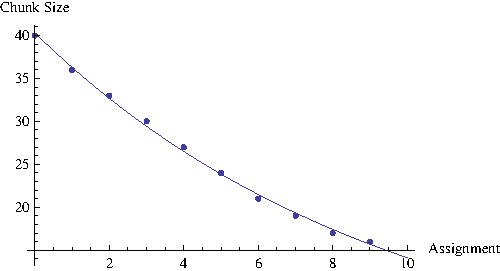
\includegraphics[width=0.7\textwidth]{fit.pdf}
  \caption{Chunk size versus assignment number, the solid line is a fit to a simple exponential.}
  \label{fig:fit}
\end{figure}

\section{OpenMP Features}
We will look at a 'paper-and-pencil' parallelisation of a piece of code. The code is given below. In the rest of this section the compiler directives should be read with \texttt{\# pragma omp}.

\lstinputlisting{openmp.c}

The code starts with a general \texttt{parallel} statement where $i, j$ is declared as private and some threshold value is set for the size of the matrix. The threshold is set because overhead of creating and suspending threads is significant for small matrix sizes, so it is advantageous to use sequential code in that case. The threshold value is left undefined. The first for loop is parallelised with a simple \texttt{for} with a static schedule. The second for loop is similar but it uses a reduction operation on the $p$ value. There is a dependency between these two loops, so the first loop cannot have a nowait. The \texttt{printf} statement is performed by a single thread, where the other threads do not have to wait at that point. The next for loop is performing a function call, where this function call has a dynamic execution time, i.e. it depends on the input. Therefore we use guided scheduling in this loop. The next loop has a dependency on $i$, this may be solved by putting a \texttt{for} in the inner loop, however all the threads will then go through the entire loop over $i$. The solution is to end the \texttt{parallel} here and use a combined \texttt{parallel for} with a \texttt{firstprivate} for the inner loop. This is however very costly, so it depends very much on the matrix size if this is advantageous. The last for loop does not have any parallelisation because the function \texttt{foo} is not known and so any dependency can occur and no parallelisation can be implemented beforehand.

\section{Conclusions}
We parallelised the heat diffusion problem using OpenMP and found a linear speedup up to 8 threads with the multithreaded code as baseline, like in the case of Pthreads. However, performance compared to the sequential code is very low for 1 thread, probably because of 'false sharing' or some other unidentified problem. Furthermore we looked at different scheduling types for the parallelisation of an upper triangular matrix, where the dynamic scheduling turned out to be most efficient. Lastly we performed a 'pencil and paper' analysis of a piece of code and tried to parallelise it. 

%%% BIBLIOGRAPHY %%%
\begin{thebibliography}{7}
\bibitem{LISA}
  http://sara.nl/systems/lisa/description
\bibitem{chunk}
  http://msdn.microsoft.com/en-us/library/b5b5b6eb(v=vs.80).aspx
\bibitem{chandra}
  R. Chandra et al., \emph{Parallel Programming in OpenMP}, Academic Press, San Diego, 2001, 62
\end{thebibliography}

\end{document}
